\section{Set Theory}
Together with logic, set theory provides a significant foundation of mathematics.

\begin{definition}
    A \underline{set} $S$ is a collection of objects, which are called the \underline{elements} of $S$.

    If $x$ is in $S$, we write $x\in S$. If not, we write $x\notin S$.

    We can sometimes list the elements of $S$ with curly braces: $$S = \left\{x_1,\,x_2,\,x_3,\,\dots\right\}$$

    The order of elements, and repetitions are ignored.
\end{definition}

You may define a set by a \emph{property} that its element must satisfy. $$A = \left\{x\in S | P(x)\right\}$$ means that the elements of $A$ are precisely those elements of $S$ for which he predicate $P(x)$ is true.

The elements of a set can be sets themselves.

\begin{definition}
    If $A$ and $B$ are sets, $A$ is called a \underline{subset} of $B$, written $A\subseteq B$, if and only if every element of $A$ is also an element of $B$.

    $$A \subseteq B \implies \forall x,\, x\in A \rightarrow x\in B$$
    
    Note: every set is a subset of itself.
\end{definition}


\begin{definition}
    Two sets are \underline{equal} if they contain the same elements.
\end{definition}

\begin{definition}
    The \underline{empty set} is the set containing no elements and is denoted by $\emptyset$. $$\emptyset = \left\{\right\}$$
\end{definition}

\subsection{Operations on Sets}
Let $A$ and $B$ be any sets.

The \underline{union} of sets $A$ and $B$, denoted $A\cup B$, is the set of all elements $x$ such that $x\in A$ or $x\in B$ (or both).

$$A\cup B = \left\{x | x \in A \text{ or } x\in B\right\}$$

The \underline{intersection} of sets $A$ and $B$, denoted $A\cap B$, is the set of all elements $x$ such that $x\in A$ and $x\in B$.
$$A\cap B = \left\{x | x\in A \text{ and } x\in B\right\}$$

The \underline{set difference} of $B$ minus $A$, denoted $B-A$, and sometimes $B \setminus A$, is the set of all elements $x$ such that $x\in B$ and $x\notin A$.
$$B - A = \left\{x | x\in B \text{ and } x\notin A\right\}$$

If the sets we are considering are all subsets of some set $U$, called the \underline{universal set}, then $U - A$ is called the \underline{complement} of $A$ and is denoted $A^c$.
$$A^c = \left\{x\in U | x\notin A\right\}$$

\subsection{More Definitions for Sets}
\begin{definition}
    For any set $S$, the \underline{power set} of $S$, denoted by $\mathcal{P}(S)$, is the set of all subsets of $S$.
    $$\mathcal{P}(S) = \left\{X | X\subseteq S\right\}$$
\end{definition}

\begin{example}
    For set $S = \left\{1,\,3\right\}$, the power set will be $\mathcal{P}(S) = \left\{\emptyset,\,\left\{1\right\},\,\left\{3\right\},\,\left\{1,\,3\right\}\right\}$
\end{example}

If $|S| = n$, then $|\mathcal{P}(S)| = 2^n$

\begin{definition}
    Two sets $A$ and $B$ are \underline{disjoint} if and only if $A\cap B = \emptyset$
\end{definition}

\begin{definition}
    Sets $A_1,\,A_2,\,A_3,\,\dots$ are \underline{mutually disjoint} (or \underline{pairwise disjoint} or \underline{nonoverlapping}) if and only if $A_i \cap A_j = \emptyset$ whenever $i\neq j$.
\end{definition}

\begin{definition}
    A finite or infinite collection of non-empty sets $\left\{A_1,\,A_2,\,A_3\,\dots\right\}$ is a \underline{partition} of a set $A$ if and only if $A$ is the union of all the $A_i$ and $A_1,\,A_2,\,A_3,\,\dots$ are mutually disjoint.
\end{definition}

\begin{definition}
    Let $n\in\mathbb Z^+$ and let $x_1,\,x_2,\,\dots,\,x_n$ be $n$ not necessarily distinct elements. The \underline{ordered n-tuple}, denoted $\left(x_1,\,x_2,\,\dots,\,x_n\right)$, consists of the $n$ elements with their ordering: first $x_1$, then $x_2$, and so on up to $x_n$.

    When $n=2$, we call this an ordered pair. When $n=3$, we call this can ordered triple.
\end{definition}

\begin{definition}
    The \underline{Cartesian Product} of sets $A$ and $B$, denoted $A\times B$ is $$A\times B = \left\{\left(a,b\right) | a\in A,\, b\in B\right\}$$
\end{definition}

\subsection{Intervals}
Given $a,b\in\mathbb R$ with $a\leq b$,
$$\left(a,b\right) = \left\{x\in\mathbb R | a < x < b\right\} \quad\text{open interval}$$

$$\left[a,b\right] = \left\{x\in\mathbb R | a \leq x \leq b\right\} \quad\text{closed interval}$$

$$\left(a,b\right] = \left\{x\in\mathbb R | a < x \leq b\right\} \quad\text{closed interval}$$ and similarly for $\left[a,b\right)$.

\subsection{Cardinality}
\begin{definition}
    The \underline{cardinality} of a set is a measure of how large it is.

    We say that two sets $X$ and $Y$ have the same cardinality if and only if there is a bijection between them. We write this as $|X| = |Y|$
\end{definition}

If $|X| = |Y|$ and $|Y| = |Z|$, then $|X| = |Z|$

A \underline{finite} set is either one which has no elements at all, or one for which there exists a bijection with a set of the form $\left\{1,\,2,\,\dots,\,n\right\}$ for some fixed positive integer $n$.

An \underline{infinite} set is a non-empty set for which there does not exist any bijection with aa set of the form $\left\{1,\,2\,\dots,\,n\right\}$ for any positive integer $n$.

\subsubsection{Finite Sets}
\begin{theorm}
    Suppose $X$ and $Y$ are finite sets.
    \begin{enumerate}
        \item if $|X|>|Y|$, then there is no injective function $f:X\rightarrow Y$
        \item if $|X|<|Y|$, then there is no surjective function $f:X\rightarrow Y$
        \item There is a bijection $f:X\rightarrow Y$ if and only if $|X|=|Y|$
    \end{enumerate}

    \underline{Corollary}: For finite sets $X$ and $Y$ with $|X|=|Y|$, the following statements are equivalent:
    $$f:X\rightarrow Y \qquad\text{is injective}$$
    $$f:X\rightarrow Y \qquad\text{is surjective}$$
    $$f:X\rightarrow Y \qquad\text{is bijective}$$
\end{theorm}

\subsubsection{Infinite Sets}
Let $2\mathbb Z = \left\{n | n = 2k\text{ for some }k\in\mathbb Z\right\}$. Prove that $|\mathbb Z| = |2\mathbb Z|$

\begin{proof}
    Define a function $f:\mathbb Z \rightarrow 2\mathbb Z$ as follows: $$f(k) = 2k \qquad\text{for every $k\in\mathbb Z$}$$

    \underline{To show f is injective}:
    Suppose $k_1,\,k_2\in\mathbb Z$ and $f(k_1) = f(k_2)$. Then $2k_1 = 2k_2$, so, by dividing both sides by 2, we have $k_1 = k_2$. Hence $f$ is injective.

    \underline{To show f is surjective}:
    Suppose $n\in 2\mathbb Z$. Then $n=2k$ for some $k\in\mathbb Z$. Hence $f(k) = 2k = n$ so $f$ is surjective.

    Thus $f$ is a bijection from $\mathbb Z$ to $2\mathbb Z$ $$\therefore |\mathbb Z| = |2\mathbb Z|$$
\end{proof}

Fact: $|\mathbb Z^+| = |\mathbb Z|$.

\begin{figure}[H]
    \centering
    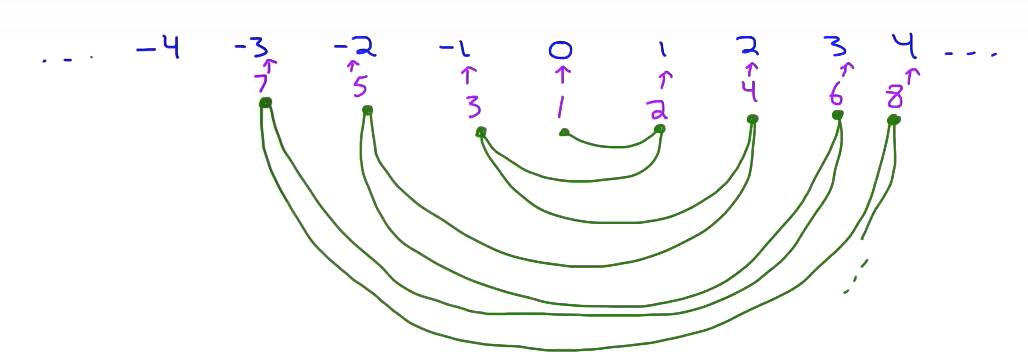
\includegraphics[width=0.5\textwidth]{z_zpos_cardinality}
\end{figure}

The function $f:\mathbb Z^+ \rightarrow \mathbb Z$ defined by $$f(n) = \frac{n}{2}\qquad \text{if $n\in\mathbb Z^+$ is even}$$ $$f(n) = -\frac{n-1}{2}\qquad \text{if $n\in\mathbb Z^+$ is odd}$$ is a bijection.

\subsection{Counting Sets}
\begin{definition}
    A set is called \underline{countably infinite} if and only if it has the same cardinality as the set of positive integers $\mathbb Z^+$
\end{definition}

\begin{example}
    $\mathbb Z$, $2\mathbb Z$, $\mathbb Q^+$, $\mathbb Q$ are all countably infinite.
\end{example}

\begin{definition}
    A set is called \underline{countable} if and only if it is finite or countably infinite. A set that is not countable is called \underline{uncountable}.
\end{definition}
\begin{theorm}
    Any subset of any countable set is countable.
\end{theorm}

Corollary: any set with an uncountable subset is uncountable.

\begin{theorm}
    The set $\left\{x\in\mathbb R | 0 < x < 1\right\}$ is uncountable.
\end{theorm}

Note: every real number between $0$ and $1$ has a unique decimal representation except that $$0.199999\dots = 0.2000\dots$$ and for such numbers, we agree to take the one that ends in all $0$'s.

\begin{proof}
    Suppose the theorem is false.
    Then $\left\{x\in\mathbb R | 0 < x < 1\right\}$ is countable, so the decimal representations of these numbers can be written in a list.
    \begin{equation*}
            \begin{array}{c}
                0.a_{11}a_{12}a_{13}a_{14}\dots a_{1n}\dots \\
                0.a_{21}a_{22}a_{23}a_{24}\dots a_{2n}\dots \\
                0.a_{31}a_{32}a_{33}a_{34}\dots a_{3n}\dots \\
                \vdots
            \end{array}
    \end{equation*}
    We now construct a new decimal number $$d = 0.d_1d_2d_3\dots d_n \dots$$ as follows \begin{equation*}
    \left\{\begin{array}{ll}
        1 & \text{if $a_{nn} \neq 1$} \\
        2 & \text{if $a_{nn} = 1$}
\end{array}\right.
    \end{equation*}

    For instance, take the above $a$ numbers as
    \begin{equation*}
            \begin{array}{c}
                0.120411\dots \\
                0.201377\dots \\
                0.135600\dots \\
                0.897124\dots \\
                \vdots
            \end{array}
    \end{equation*}

    So $$d = 0.2112\dots$$ Note that for each integer $n\in\mathbb Z^+$, $d$ differs from the n\ts{th} real number in the list because it differs in the n\ts{th} decimal place.

    Thus, $d\in\left\{x\in\mathbb R | 0 < x < 1\right\}$ but $d$ does not belong to the list of all real numbers between $0$ and $1$, which is a contradiction.

    Therefore $\left\{x\in\mathbb R | 0 < x < 1\right\}$ is uncountable.
\end{proof}

This shows that since $\left(0,1\right)\subseteq \mathbb R$ and $\left(0,1\right)$ is uncountable, $\mathbb R$ is uncountable.

\subsubsection{Comparing Cardinalities}
\begin{enumerate}
    \item $|X| \leq |Y|$ if and only if $\exists$ injective $f:X\rightarrow Y$
    \item $|X| \geq |Y|$ if and only if $\exists$ surjective $f:X\rightarrow Y$
    \item $|X| < |Y|$ if and only if \begin{enumerate}
        \item $\exists f:X\rightarrow Y$ such that $f$ is injective
        \item $\nexists f:X\rightarrow Y$ such that $f$ is bijective
    \end{enumerate}
    \item $|X| > |Y|$ if and only if \begin{enumerate}
        \item $\exists f:X\rightarrow Y$ such that $f$ is surjective
        \item $\nexists f:X\rightarrow Y$ such that $f$ is bijective
    \end{enumerate}
\end{enumerate}

\begin{definition}
    $|\emptyset| < |X|$ and $|X| > |\emptyset|$ for all $X\neq \emptyset$
\end{definition}

\subsubsection{The Schroder-Bernstein Theorm}
If $|X| \leq |Y|$ and $|X| \geq |Y|$, then $|X| = |Y|$.

Thus, to show $|X| = |Y|$, it is enough to find
\begin{enumerate}
    \item an injective function $X\rightarrow Y$ and
    \item a surjective function $X\rightarrow Y$
\end{enumerate}
OR
\begin{enumerate}
    \item an injective function $X\rightarrow Y$ and
    \item an injective function $Y\rightarrow X$
\end{enumerate}
OR
\begin{enumerate}
    \item a surjective function $X\rightarrow Y$ and
    \item a surjective function $Y\rightarrow X$
\end{enumerate}

This can be much easier than finding a bijection.

\begin{example}
    Show $|\mathbb Z^+| = |\mathbb Q^+|$ using the Schroder-Bernstein theorem.

    \begin{enumerate}
        \item The function $f:\mathbb Z^+ \rightarrow Q^+$ is defined by $f(n) = n\,\forall n\in\mathbb Z^+$ is injective $\therefore |\mathbb Z^+| \leq |\mathbb Q^+|$
        \item Let $g:\mathbb Q^+ \rightarrow \mathbb Z^+$ be defined as follows: for each $q\in\mathbb Q^+$, let $q = \frac{a}{b}$ where $a,b\in\mathbb Z^+$, $b\neq 0$ and $\text{gcd}(a,b)= 1$ and let $g(q) = 2^a 3^b$.
    \end{enumerate}

    Proof that $g$ is injective:

    Let $q_1 = \frac{a}{b}$ and $q_2 = \frac{c}{d}$ as described above and suppose $g(q_1) = g(q_2)$. Then $2^a 3^b = 2^c 3^d$. By unique prime factorisation, $a=c$ and $b=d$. Hence, $q_1=q_2$ so $g$ is injective. $\therefore |\mathbb Q^+| \leq |\mathbb Z^+|$.
\end{example}

\subsection{Relations on Sets}
\begin{definition}
    Given sets $A$ and $B$, a \underline{binary relation} $R$ from $A$ to $B$ is a subset of $A\times B$. If $(x,y)\in\mathbb R$ we also write $xRy$ and say that $x$ is \underline{related} to $y$. Other symbols may be used to denote a relation ($\rho, \sigma, \tau,$ etc)
\end{definition}

\begin{definition}
    If $R$ is a binary relation from $A$ to $B$, the the \underline{inverse relation} $R^{-1}$ is defined from $B$ to $A$ by $$R^{-1} = \left\{(b,a)\in B\times A | (a,b)\in R\right\}$$

    So for all $a\in A$ and $b\in B$, $$(b,a)\in R^{-1} \text{ if and only if }(a,b)\in R$$
\end{definition}
A relation on a set A, is a relation from A to A.\\
\newpage
\begin{definition}
    Let R be a relation on a set A.\\
    \begin{enumerate}
        \item R is reflexive if and only if \(\forall x \in A, ~~xRx\)
        \item R is symmetric if and only if \(\forall x,y \in A\) if \(xRy\) then \(yRx\)
        \item R is transitive if and only if \(\forall x,y,z \in A\) if \(xRy\) and \(yRz\), then \(xRz\)
    \end{enumerate}
\end{definition}
Note that a relation R on a set A is symmetric if and only if \(R = r^{-1}\).\\
\begin{definition}
    R is an equivalence relation if R is symmetric, reflexive and transitive.
\end{definition}
\begin{definition}
    Let R be an equivalence relation on a set A and let \(a \in A\).\\
    The equivalence class of a is \[[a] = \{x\in A | xRa\}\]
    So, \(\forall x\in A\quad x\in [a] \iff xRa\)
\end{definition}
\begin{theorm}
    If R is an equivalence relation on a set A and \(a, b \in A\) satisfy \(aRb\), then \([a] = [b]\).
\end{theorm}
\begin{theorm}
    If R is an equivalence relation on a set A and \(a, b \in A\) and \([a] \cap [b] \neq \emptyset\) then \([a] = [b]\).
\end{theorm}
\begin{theorm}
    If R is an equivalence relation on a set A then the set of equivalence classes of R forms a partition of A. That is, the union of all the classes is A and the intersection of any two distinct classes is empty.\\
    Given a partition of a set A, the binary relation R induced by the partition is defined:\\
    for all \(x, y \in A\), \(xRy \iff\) there is a set in the partition containing both x and y.
\end{theorm}
\begin{theorm}
    Given a partition of a set A, and the binary relation R, induced by the partition, it follows that R is reflexive, symmetric and transitive.
\end{theorm}
\begin{definition}
    A relation R on a set A is antisymmetric if and only if \(\forall a, b \in A\) if \(aRb\) and \(bRa\) then \(a=b\)
\end{definition}
\begin{definition}
    Let R be a relation on a set A. Elements \(a, b\in A\) are comparable if and only if \(aRb\) or \(bRa\). Otherwise, a and b are non-comparable.
\end{definition}
\begin{definition}
    Let R be a relation on a set A. R is a total order relation if and only if, R is a partial order relation such that all elements are comparable.\\
    That is, R is a total order relation if and only if: Reflexive, antisymmetric, transitive and \(\forall a, b \in A\) either \(aRb\) or \(bRa\).
\end{definition}
